\documentclass[UTF8]{article}
\usepackage{ctex}
\usepackage{geometry}
\usepackage{float}
\usepackage{graphicx}
\usepackage{listings}
\usepackage{subfigure}
\usepackage{amsmath}
\geometry{a4paper,left=2cm,right=2cm,top=2cm,bottom=2cm}
\title{气流速度测量实验}
\author{能动A71 宋德培 2174110112}

\renewcommand{\thesection}{\Roman{section}}
\renewcommand{\thesubsection}{\arabic{section} .\arabic{subsection}}
\usepackage{xcolor}
\lstset{
	numbers=left, 
	numberstyle= \tiny, 
	keywordstyle= \color{ blue!70},
	commentstyle= \color{red!50!green!50!blue!50}, 
	frame=shadowbox, % 阴影效果
	rulesepcolor= \color{ red!20!green!20!blue!20} ,
	escapeinside=``, % 英文分号中可写入中文
	xleftmargin=2em,xrightmargin=2em, aboveskip=1em,
	framexleftmargin=2em
} 
\begin{document}
	\maketitle
	\section{实验目的}
	\begin{enumerate}
	\item	通过实验, 掌握利用空气动力探针测量风管内气流速度的方法,以及相关仪器仪表的使用。。
	\item 	通过实验,掌握毕托管和三孔探针测量气流速度的原理,并了解其结构。。
	\end{enumerate}
	
	\section{实验原理}
	\subsection{毕托管测速}
	毕托管在正对来流方向时,可分别别测得流体总压以及静压,根据总压与静压间的关系,使用毕托管测得动压后,可直接从公式
	\[
	v=\sqrt{\frac{2}{\rho}p_dk_u}
	\]
	得到流体速度。其中$k_u$为标定系数,与静压孔形状和位置、头部形状等因素有关。
	\subsection{三孔探针测速}
	当三孔探针正对来流方向时,两个侧孔压差为零,从中心孔与侧孔压差可以表示为
	\[
	p_2-p_1=\frac{\rho}{2}v^2(k_0-k_1)=\Delta h_{2-1}
	\]
	因此可以求出气流速度
	\[
	v=\sqrt{\frac{2\Delta h_{2-1}}{\rho(k_0-k_1)}}
	\]
	而总压也可以计算得到
	\[
	\begin{split}
	p_0&=\frac{\rho}{2}v^2+\Delta h_2-\frac{k_0}{k_0-k_1}\Delta h_{2-1}\\
	&= \Delta h_2-\frac{1-k_0}{k_0-k_1}\Delta h_{2-1}
	\end{split}
	\]
	其中$k_0,k_1$分别为中心孔和侧孔的标定系数。
	\section{数据记录及处理}
	\subsection{\textit{原始数据记录}}
	\begin{figure}[H]
		\centering
		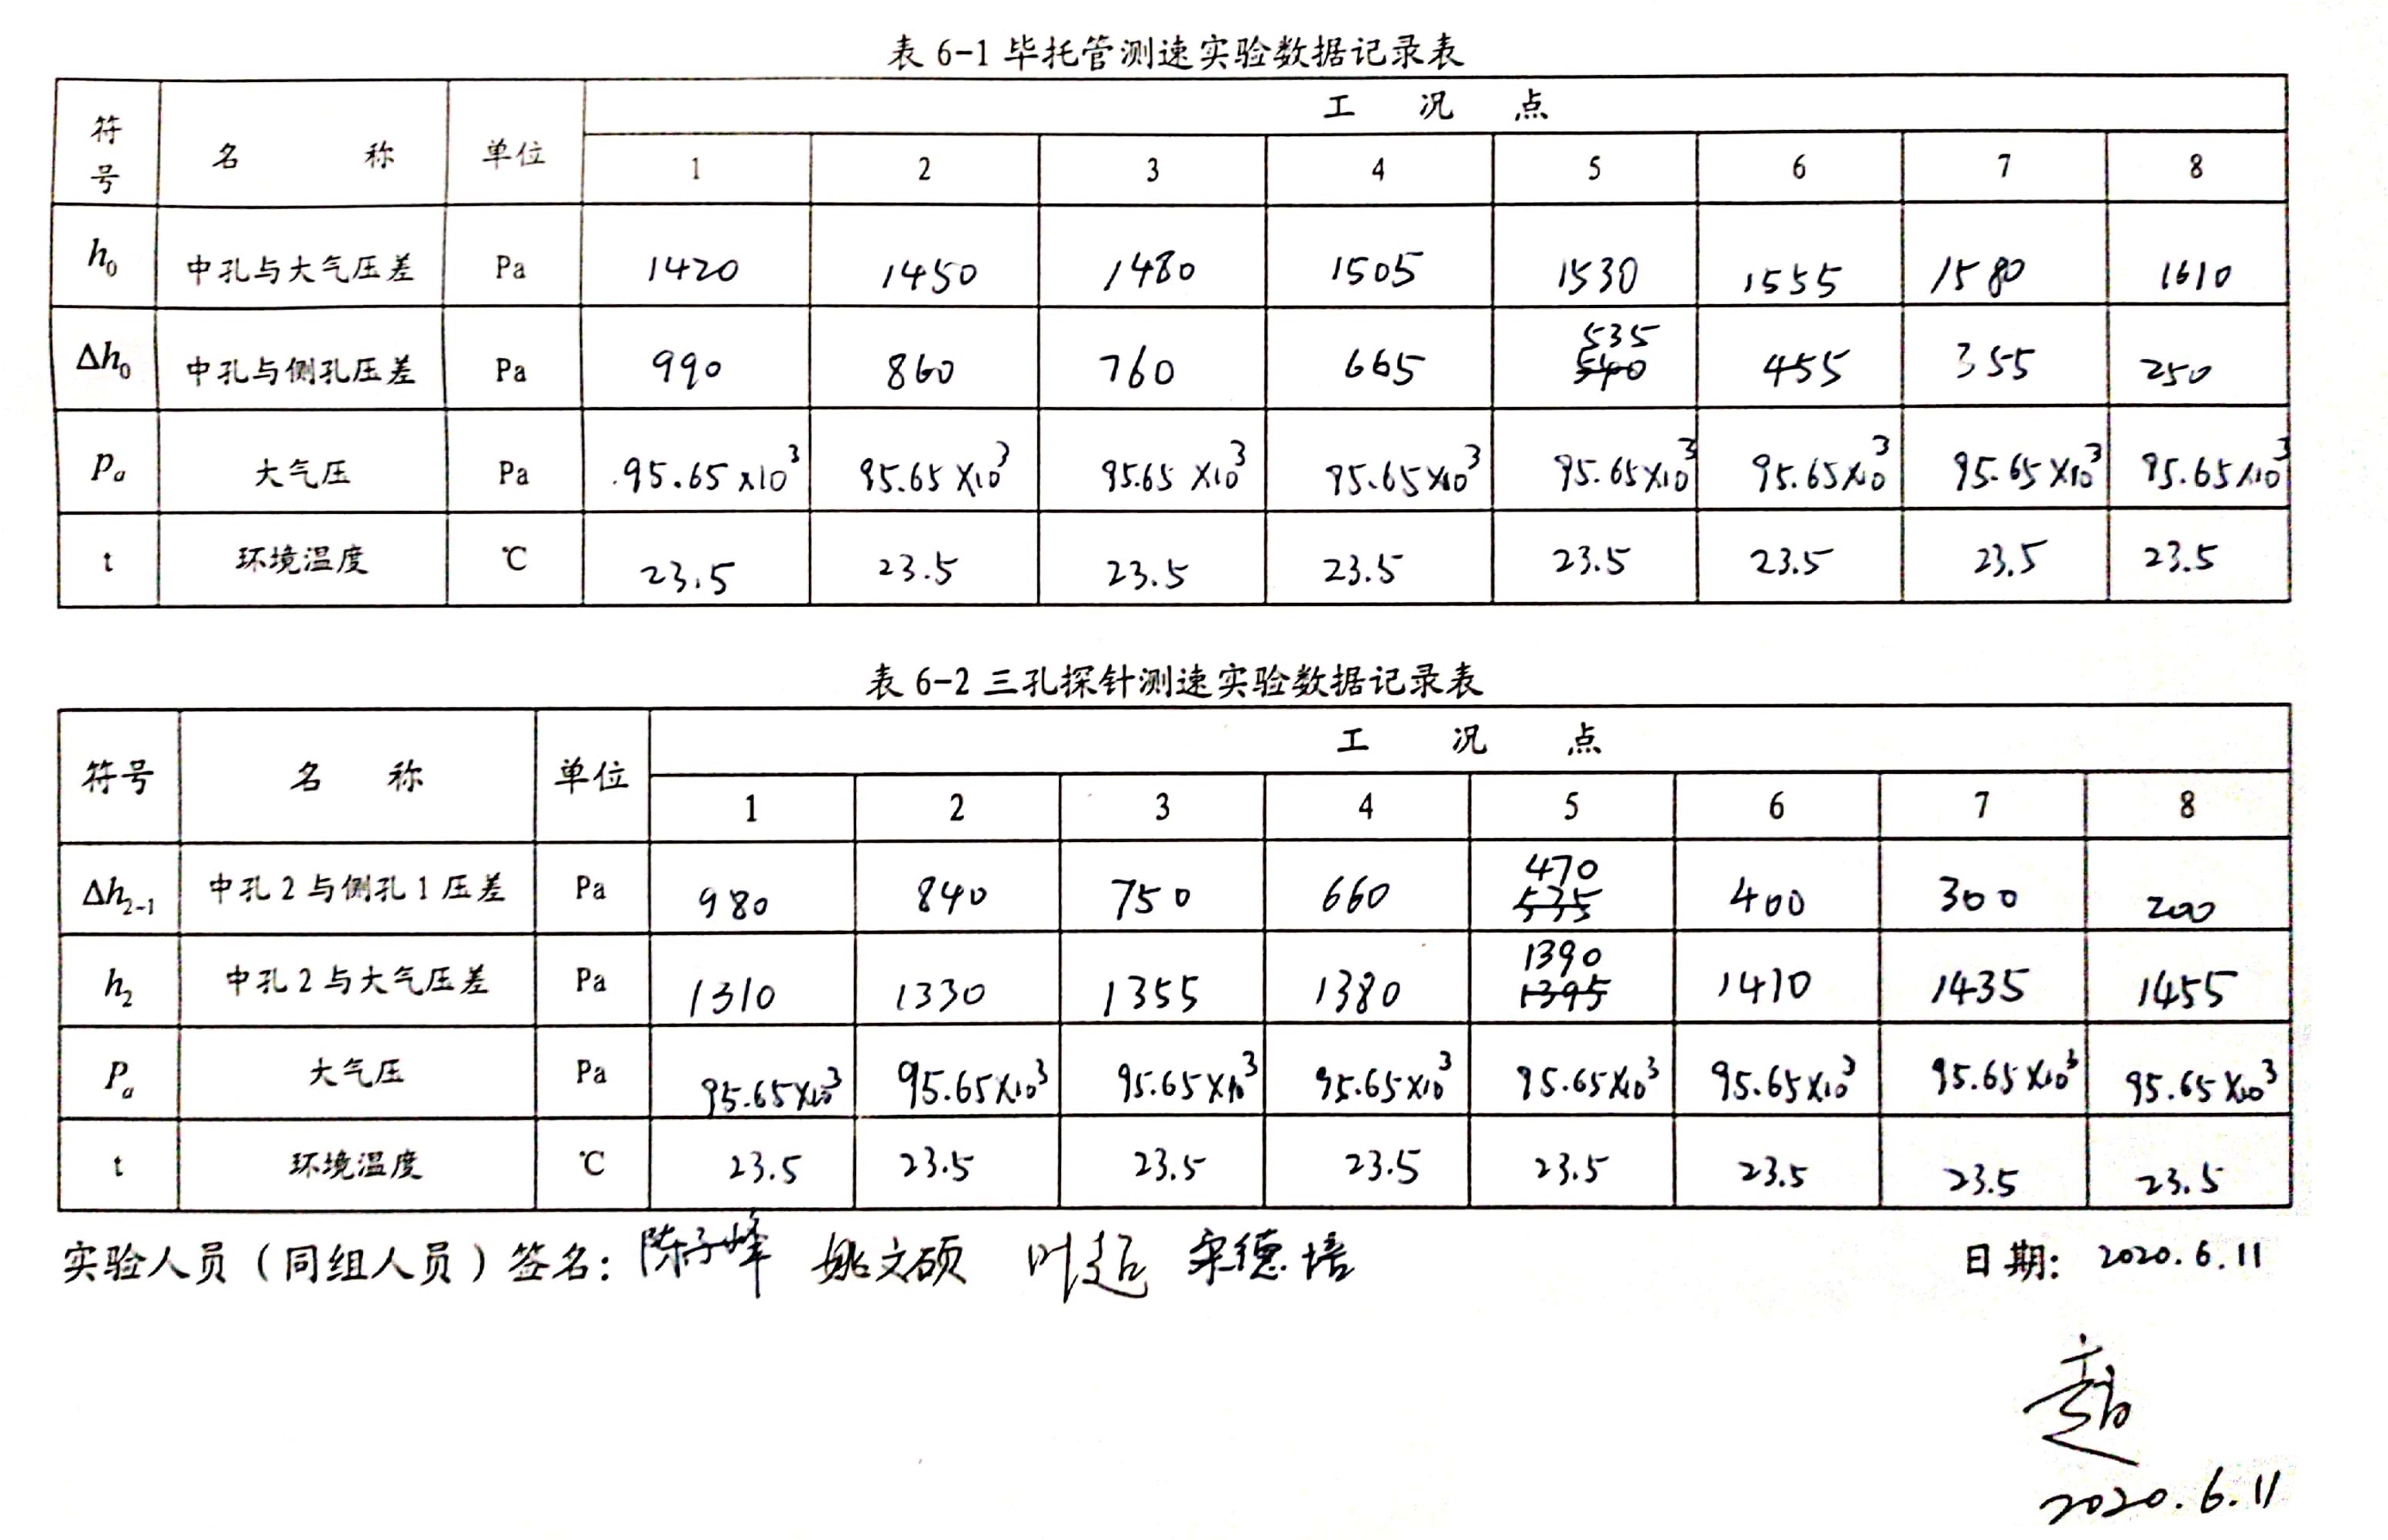
\includegraphics[width=\linewidth]{figure/origin}
		\label{fig:origin}
	\end{figure}
	\subsection{\textit{数据处理}}
	\begin{figure}[H]
		\centering
		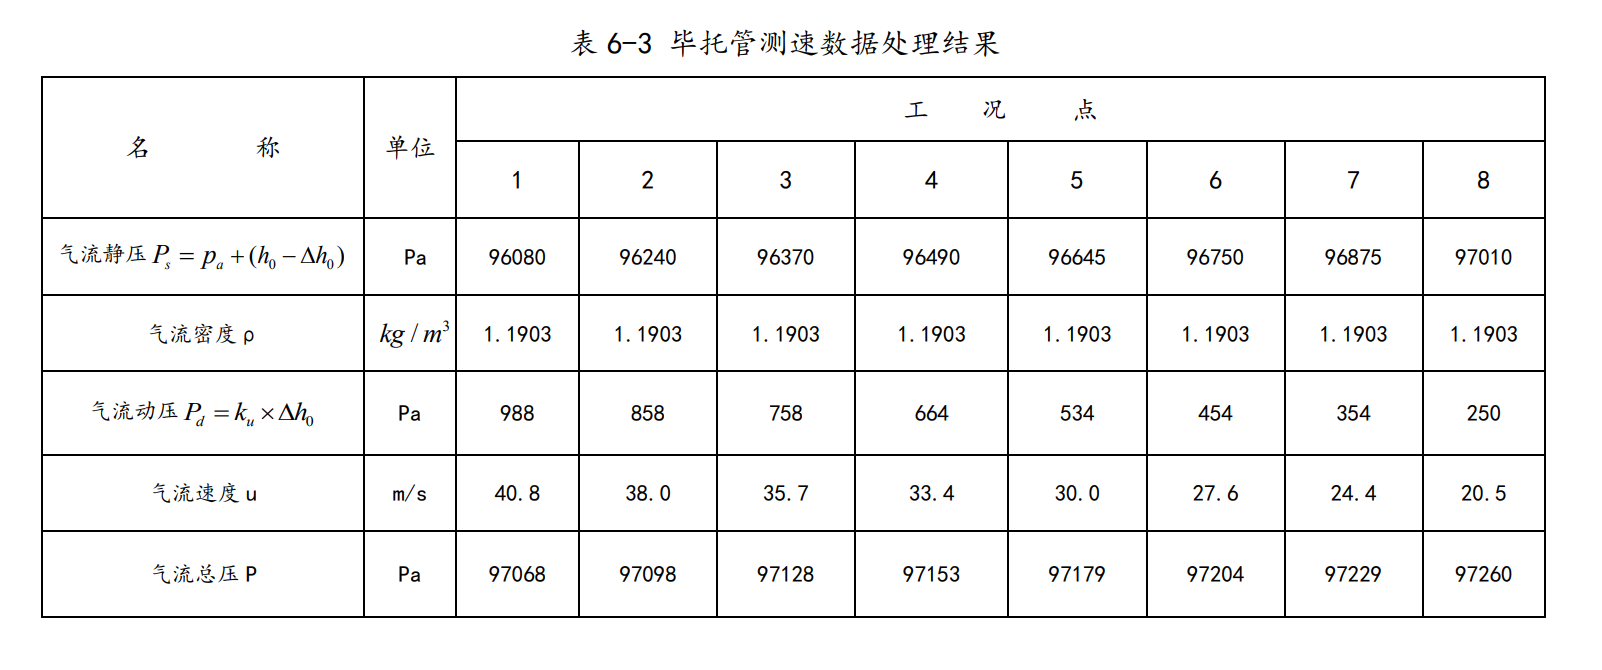
\includegraphics[width=0.9\linewidth]{figure/fig1}
		\label{fig:fig1}
	\end{figure}
	\begin{figure}[H]
		\centering
		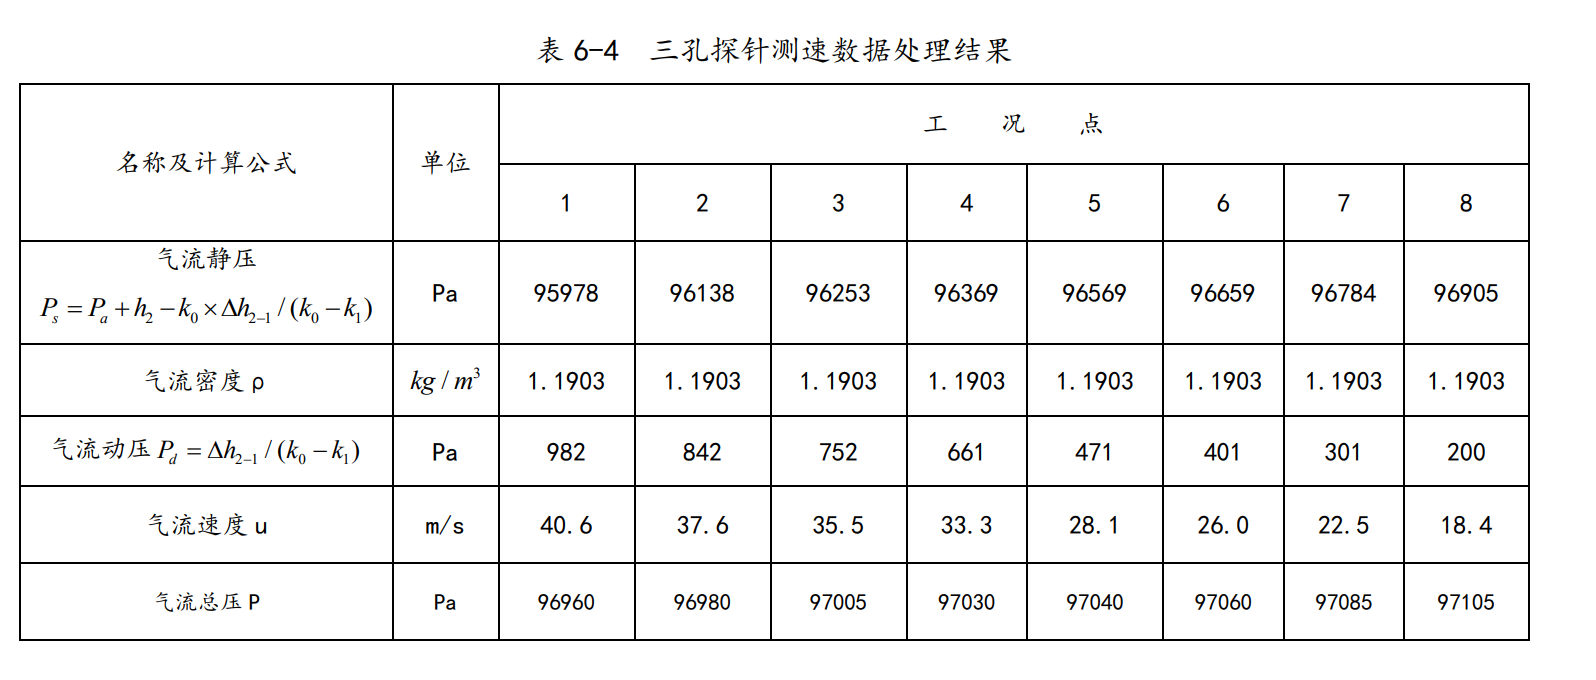
\includegraphics[width=0.9\linewidth]{figure/fig2}
		\label{fig:fig2}
	\end{figure}
	
	\begin{figure}[H]
		\centering
		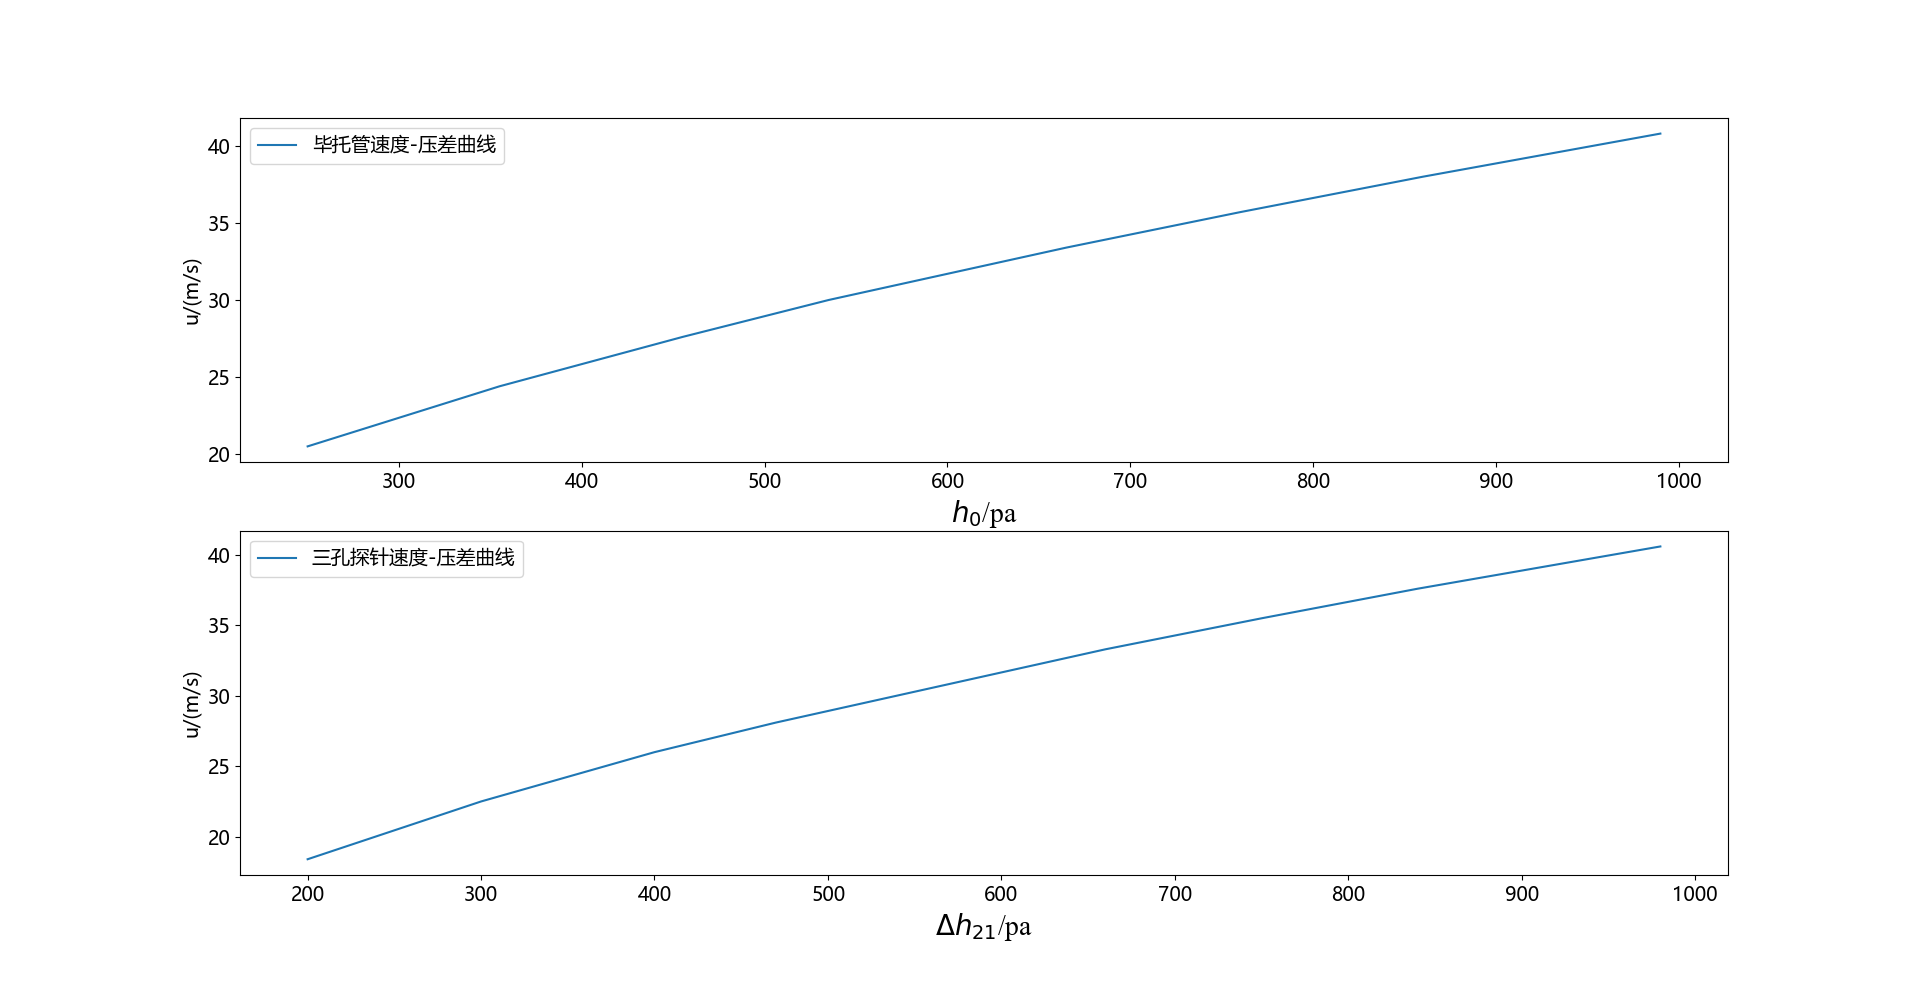
\includegraphics[width=\linewidth]{figure/Figure_1}
		\caption{毕托管及三孔探针速度-压差曲线}
		\label{fig:figure1}
	\end{figure}
	\section{实验结果分析}
	\textbf{1.	什么是气流总压和气流静压?它们之间有什么关系?}
	
	在被物体绕流时,物体上有些点上流体完全滞止,即速度为零,这些点上的压力为滞止压力,也称流体总压;同样另一类点,流体压力等于未扰动流体的压力(静压),这些点的压力为流体静压。两者存在关系式
	\[
	p_0 = \frac{\rho}{2}v^2+p_s
	\]
	
	\textbf{2.	毕托管和三孔探针各有何优缺点?}
	
	毕托管结构简单,使用方便,稳固可靠,并且只要精心制造并经过严格标定可以实现较高测量精度,但是在测量时必须正对来流方向,无法测量气流方向。
	
	三孔探针结构和操作较为复杂,非正对气流方向需要查表,但是可以同时测量气流速度大小与方向。
	
	\textbf{3.	影响测量精度的因素有哪些?}
	
	\begin{itemize}
		\item 测量时三孔探针中心孔以及毕托管是否正对来流方向
		\item 测量时压差是否达到稳定
		\item 测量时环境温湿度的变化带来误差
		\item 风机出口气流的脉动现象带来误差
	\end{itemize}

	\textbf{4.	分析测量误差和曲线图。}
	
	从实验数据处理结果可以看出,毕托管和三孔探针测量得到的动、静压差非常接近,计算得到的速度也较为接近,误差较小。实验误差在流速较小时增大,分析原因可能是因为在阀门开度减小,气流速度减小时,管内气流流场被破坏,湍动度增大,使得速度脉动增大,因此引起误差增加。为了增加实验精度,可以在每次调节开度后增加等待时间,待流场稳定后再进行读数。
	
	\textbf{5.	实验体会:实验中遇到了哪些问题?是如何解决的?}
	
	实验中发现三孔探针的1、3孔平衡较难调节,因为系统有惯性,旋转探针后过一段时间显示的压力才会变化,因此在调节过程中,缓慢调节,变调节边观察测压计液面变化,最终使得两个孔的压差大致为零。
	
\end{document}